\documentclass[thesis.tex]{subfiles}

\begin{document}
\onlyinsubfile{\setcounter{section}{0}}
\onlyinsubfile{\subfilefrontmatter}
\section{Introduction}\label{sec:introduction}

%% File paths are relative to the output PDF in the build directory, but only when building with subfiles...
% !TeX root = ../introduction.tex
\section{Neural Networks}\label{sec:introduction:neural-networks}

Much of the future discussion on neural network language models will require at least an intuitive understanding of neural networks.
This section aims to provide enough background and vocabulary to facilitate discussion of neural networks as a concept without becoming bogged down in a nontrivial amount of detail.
\begin{figure}[h]
    \centering
    
\includegraphics[scale=0.5]{machine_learning}
    \caption{The pile gets soaked with data and starts to get mushy over time, so it's technically recurrent \cite{xkcd_machine_learning}}\label{fig:neural-networks:xkcd-machine-learning}
\end{figure}
There are many other excellent introductions to neural networks that provide much more detail such as \cite{goodfellow_bengio_courville_2016} for a general mathematical treatment, or \cite{goldberg_2017} for a treatment specific to processing natural language.
\TODO{This information is provided purely to ensure a consistent vocabulary, and has been produced without reference material. It should be fact-checked and appropriately cited.}

\subsection{A Biological Metaphor}\label{sec:neural-networks-biological-metaphor}

If our intent is to produce intelligent, sophisticated statistical models, it is useful to motivate our model with the biological metaphor of a single neuron.
Of course, our intent is not to emulate, nor is it to simulate a collection of biological neurons.
We simply wish to motivate a mathematical discussion of a statistical model that has proved useful in data analysis, modeling, and prediction.
In this spirit, we note that it is well beyond the scope of this paper to provide a biologically correct description of the hugely complex field of neuroscience.
In fact, it would be reasonable to present neural networks devoid of any biological motivation simply as a mathematical model that has proven to be useful.

\begin{figure}[h]
    \centering
    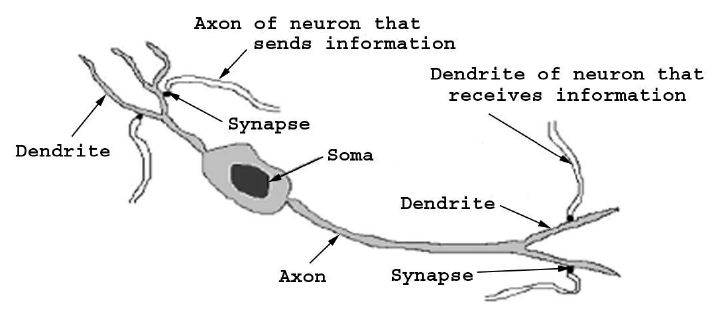
\includegraphics[scale=0.5]{biological_neuron}
    \caption{A biological neuron \cite{bio_neuron}}\label{fig:neural-networks:biological-neuron}
\end{figure}

\autoref{fig:neural-networks:biological-neuron} shows a ``typical'' neuron (of course there is no such thing) with various labeled components.
In the most general sense, a neuron takes in input through its dendrites, processes the received information, and under the right conditions emits a signal through its axon to the dendrites of an adjacent neuron \cite{bio_neuron}.
Somehow, through an organization of many such neurons, intelligent behavior emerges \cite{castro_2006}.

Even such a grossly simplified treatment of a neuron provides motivation for the artificial neuron shown in \autoref{fig:neural-networks:artificial-neuron}.
\begin{figure}[h]
    \centering
    \begin{tikzpicture}[
        node distance=3cm,
        >={Stealth[length=2mm]},
        ]

        \node[draw, circle, label=below:{activation}] (unit) {$\sum\quad f$};
        \draw[dashed] (unit.north) -- (unit.south);

        \node[draw, circle, above left=2.1cm of unit] (x_0) {$x_0$};
        \node[draw, circle, below=5mm of x_0] (x_1) {$x_1$};
        \node[draw, circle, below=5mm of x_1] (x_2) {$x_2$};
        \node[below=1mm of x_2] (dots) {$\vdots$};
        \node[draw, circle, below=3mm of dots, label=below:{input}] (x_n) {$x_n$};

        \node[draw, circle, right=3cm of unit, label=below:{output}] (output) {$y$};

        \draw[->] (x_0) -- node[midway, sloped, above] {$w_0$} (unit);
        \draw[->] (x_1) -- node[midway, sloped, above] {$w_1$} (unit);
        \draw[->] (x_2) -- node[midway, sloped, above] {$w_2$} (unit);
        \draw[->] (x_n) -- node[midway, sloped, above] {$w_n$} (unit);
        \draw[->] (unit) -- node[midway, above] {$f\left(\sum_{i=1}^n w_ix_i \right)$} (output);

    \end{tikzpicture}
    \caption{An artificial neuron}\label{fig:neural-networks:artificial-neuron}
\end{figure}
The artificial neuron, called a \textit{unit}, takes a fixed number of inputs $x_0, \dots, x_n$, multiplies each with its corresponding weight, and adds the weighted inputs together before piping the result through the activation function $f$.
Note that if the inputs are treated as a column vector $\vec x$, and the weights as a vector $\vec w$, the output is the result of the operation
\begin{equation*}
    y = f(\vec w \cdot \vec x)
\end{equation*}
Often it is useful to add a bias term $b$
\begin{equation}
    y = f(\vec w \cdot \vec x + b) \label{eq:neural-networks:ffnn-unit}
\end{equation}
by adding a fixed unitary input to the neuron as in \autoref{fig:neural-networks:artificial-neuron-bias}.
This allows us to treat the bias term exactly like one of the weights when assembling multiple such units together to form a network.
\begin{figure}[h]
    \centering
    \begin{tikzpicture}[
        node distance=3cm,
        >={Stealth[length=2mm]},
        ]

        \node[draw, circle, label=below:{activation}] (unit) {$\sum\quad f$};
        \draw[dashed] (unit.north) -- (unit.south);

        \node[draw, circle, above left=2.1cm of unit] (one) {$+1$};
        \node[draw, circle, below=5mm of one] (x_0) {$x_0$};
        \node[draw, circle, below=5mm of x_0] (x_1) {$x_1$};
        \node[below=1mm of x_1] (dots) {$\vdots$};
        \node[draw, circle, below=3mm of dots, label=below:{input}] (x_n) {$x_n$};

        \node[draw, circle, right=3cm of unit, label=below:{output}] (output) {$y$};

        \draw[->] (one) -- node[midway, sloped, above] {$b$} (unit);
        \draw[->] (x_0) -- node[midway, sloped, above] {$w_0$} (unit);
        \draw[->] (x_1) -- node[midway, sloped, above] {$w_1$} (unit);
        \draw[->] (x_n) -- node[midway, sloped, above] {$w_n$} (unit);
        \draw[->] (unit) -- node[midway, above] {$f(\vec w \cdot \vec x + b)$} (output);

    \end{tikzpicture}
    \caption{An artificial neuron with a unitary bias input}\label{fig:neural-networks:artificial-neuron-bias}
\end{figure}

Presumably then, the intelligence of a neural network has something to do with how the units are assembled together, and with the magical weight values associated with each unit.
Unlike the chaotic and organic layout in the human body, we assemble the artificial neurons into sequential layers, and connect the outputs of the previous layer to the inputs of the next.

\begin{figure}[h]
    \centering
    \begin{tikzpicture}[scale=1.8, >={Stealth[length=2mm]},->, draw=black!50, node distance=3cm]
        \tikzstyle{every pin edge}=[<-]
        \tikzstyle{neuron}=[draw, black, thick, circle, minimum size=1cm, inner sep=0pt]
        \tikzstyle{annot} =[text width=4em, text centered]

        % Draw the input layer nodes
        \foreach \name / \y in {0,...,3}
        \node[neuron, pin=left:{$x_\y$}] (I-\name) at (0,-\y-1) {};

        % Draw the hidden layer nodes
        \foreach \name / \y in {1,...,5}
        \path[yshift=0.5cm]
        node[neuron] (H-\name) at (2.5cm,-\y cm) {};

        % Draw the output layer node
        \node[neuron,pin={[pin edge={->}]right:{$y$}}, right of=H-3] (O) {};

        % Connect every node in the input layer with every node in the hidden layer.
        \foreach \source in {0,...,3}
        \foreach \dest in {1,...,5}
        \path (I-\source) edge (H-\dest);

        % Connect every node in the hidden layer with the output layer
        \foreach \source in {1,...,5}
        \path (H-\source) edge (O);

        % Annotate the layers
        \node[annot,above of=H-1, node distance=1cm] (hl) {Hidden layer};
        \node[annot,left=2.5cm of hl] {Input layer};
        \node[annot,right of=hl] {Output layer};
    \end{tikzpicture}
    \caption{Multiple units arranged into a network}\label{fig:neural-networks:multilayer-perceptron}
\end{figure}

When we treat the cells as a vertical layer, \autoref{eq:neural-networks:ffnn-unit} becomes
\begin{equation}
    \vec y = f(W^T \vec x + \vec b) \label{eq:neural-networks:ffnn-layer}
\end{equation}
where each of the weight vectors $\vec w$ for each cell is arranged into the matrix $W$, and each of the $y$-values are concatenated to form $\vec y$.
Common choices for the activation function $f$ are the hyperbolic tangent, sigmoid, rectified linear unit, and softmax functions.
Note that the use of $f$ in \autoref{eq:neural-networks:ffnn-layer} assumes that the same activation function is used for every unit in the layer.

Due to the large amount of homogeneity in the units for each layer, we almost never draw schematic diagrams of a network's architecture showing the individual units.
Instead, we treat the layer of units as the basic abstraction as in \autoref{fig:neural-networks:architecture}.
\begin{figure}[h]
    \centering
    \begin{tikzpicture}[
        node distance=2.6cm,
        >={Stealth[length=2mm]},
        layer/.style={draw, minimum width=1cm},
        input/.style={draw, dashed, minimum height=1cm, minimum width=0.8cm}
        ]

        \node[input] (x_0) {$x_0$};
        \node[input, below=1mm of x_0, anchor=north] (x_1) {$x_1$};
        \node[below=3mm of x_1, anchor=north] (ellipsis) {$\vdots$};
        \node[input, below= 3mm of ellipsis, anchor=north] (x_n) {$x_{n_1}$};

        \node[left=1cm of x_0] (x_0_label) {$x_0$};
        \node[left=1cm of x_1] (x_1_label) {$x_1$};
        \node[left=1cm of x_n] (x_n_label) {$x_{n_1}$};

        \node[layer, fit={(x_0) (x_1) (ellipsis) (x_n)}, label=below:{$\vec x$}, label=above:{$n_1$}] (input) {};

        \node[layer, label=below:{$\tanh$}, label=above:{$n_2$}, right of=input, minimum height=4cm] (hidden) {};
        \node[layer, label=below:{softmax}, label=above:{$n_3$}, right of=hidden, minimum height=7cm] (softmax) {};
        \node[right=1.2cm of softmax] (output) {$\vec y$};

        \draw[->] (x_0_label) -- (x_0);
        \draw[->] (x_1_label) -- (x_1);
        \draw[->] (x_n_label) -- (x_n);

        \draw[->] (input) -- node[midway, above]{$W_1$} (hidden);
        \draw[->] (hidden) -- node[midway, above]{$W_2$} (softmax);
        \draw[->] (softmax) -- (output);
    \end{tikzpicture}
    \caption{An example neural network architecture diagram}\label{fig:neural-networks:architecture}
\end{figure}
The dimension of each layer is shown at the top of each layer, and the activation function of the non-input layers is indicated below each layer.
The underlying mathematical operation that this architecture defines is
\begin{equation*}
    \vec y = \softmax\left(W_2^T \tanh(W_1^T \vec x + \vec{b_1}) + \vec{b_2}\right)
\end{equation*}
where $\vec{b_1}$ and $\vec{b_2}$ are the implicit bias vectors, and $W_1$ and $W_2$ are the weight matrices for the $\tanh$ and $\softmax$ layers respectively.

Here, the softmax activation function
\begin{equation}
    \softmax(\vec x)_i = \frac{e^{x_i}}{\sum_{j=1}^n e^{x_j}} \quad \text{for each $i=1, \dots, n$} \label{eq:neural-networks:softmax}
\end{equation}
is applied element-wise to the vector $\vec x$, and produces the vector $\vec y$ which can be treated as a probability distribution over $n$ values.
That is, the vector $y$ sums to 1.
The softmax activation function is often used in neural networks whose output is to be treated as a probability, and will be used extensively in language modeling.

\TODO{Add a \textit{brief} discussion on datasets, objective functions, and optimization methods.}

% !TeX root = ../introduction.tex
\section{Modeling Natural Language}\label{sec:introduction:language-models}

Natural language in its textual form may be represented as a sequence of tokens.
The specific granularity of these token sequences varies from the coarsest word level, to individual characters, to different variations of subword morphemes, token metadata tags (like its grammatical part of speech), and punctuation.
A Language Model (LM) is a statistical model of natural language that generates a probability distribution for these sequences \cite{pappas_meyer_2012,goldberg_2017}.

In particular, given a sequence of words $w_{1:n}$, we wish to estimate the probability $P(w_{1:n})$.
In the general case, we can use the probability chain rule
\begin{equation}
    P(w_{1:n}) = P(w_n \mid w_{1:n - 1}) \cdot P(w_{n - 1} \mid w_{1:n - 2}) \cdots P(w_2 \mid w_1) \cdot P(w_1)\label{eq:language-models:chain-rule}
\end{equation}
to confirm our intuition that a language model's understanding of a given word in a sequence relies on an understanding of the full context from the current word all the back to the first word in the sequence.
That is, understanding future tokens in a sequence requires understanding not only the present, but also the entire past history of the sequence.

Of course, with any probabilistic model, we must have a method of scoring the model.\sarcasm{
    The best intuitive explanations of perplexity and its relation to entropy are \url{https://leimao.github.io/blog/Entropy-Perplexity/} and \url{https://stats.stackexchange.com/questions/10302/what-is-perplexity}}\sarcasm{
    Footnotes marked with roman numerals are for personal remarks by the author, and will be removed before submission.
}
In Shannon's seminal work on information theory \cite{Shannon1948} he discussed modeling an information source inherent information using entropy.
In the discrete case, \textit{Shannon entropy} is defined as
\begin{equation}
    \entropy(p) = - \sum_{i=1}^n p(x_i) \log_b p(x_i) \label{eq:language-models:entropy}
\end{equation}
where $p(x_i)$ is the probability of state $x_i$, and $\sum_i p(x_i) = 1$.
Entropy can be interpreted as the information content of the modeled information source.

Then the \textit{cross entropy} of two distributions $p$ and $q$ can be defined in the discrete case as
\begin{equation}
    \entropy(p, q) =  - \sum_{i=1}^n p(x_i) \log_b q(x_i) \label{eq:language-models:cross-entropy}
\end{equation}
Cross entropy can be thought of as a measure of the difference between two probability distributions \cite{ManningSchuetze99}.
Thus, cross entropy is often used as an objective function in optimization tasks, because we want to minimize the difference between the probability distribution of the training set (as an estimate of the \textit{true} probability distribution of the whole), and the distribution of the statistical model's output.

\textit{Perplexity} is defined \cite{ManningSchuetze99} as
\begin{equation}
    \perplexity(p) = b^{- \sum_{i=1}^n p(x_i) \log_b p(x_i)} \label{eq:language-models:perplexity-defn}
\end{equation}
which is precisely $b^{\entropy(p)}$, or the exponentiation of Shannon entropy!\sarcasm{
    Due to its similarity, \cite{ManningSchuetze99} supposes that perplexity is preferred over cross-entropy as a performance metric due to the more impressive nature of being able to claim large reductions in perplexity as opposed to a cross-entropy loss of a fraction of a bit.}

However, when scoring a language model, we rarely (if ever) know the true probability distribution of the language a dataset it sampled from.
So we modify \autoref{eq:language-models:perplexity-defn} to approximate the perplexity of a language model from the training set probability distribution $\tilde p$, and the language model's output distribution
\begin{equation}
    \widetilde{\perplexity}(\tilde p, \model)  = b^{- \sum_{i=1}^{n} \tilde{p}(w_i) \log_b \model(w_i)}\label{eq:language-models:perplexity-p-model}
\end{equation}
where our training dataset is formed of $n$ words $w_1, \dots, w_n$.
But the word $w_i$ is sampled uniformly from the dataset, so $\tilde p(w_i) = \frac{1}{n}$, which results in the definition of perplexity that \cite{goldberg_2017} gives.
\begin{equation}
    \perplexity(\model) = 2^{-\frac{1}{n}\sum_{i=1}^n \log_2 \model(w_i \mid w_{1:i-1})} \label{eq:language-models:perplexity}
\end{equation}

Notice that the worst possible language model would be a random choice of the next token in a sequence with a uniform distribution.
Such a model would have each $\model(w_i \mid w_{1:i-1}) = \frac{1}{n}$, which would result in a high perplexity score.
A good language model --- one that is reflective of ``real'' language --- will assign high probabilities to observed events in the test corpus, which results in minimizing the perplexity score \cite{goldberg_2017}.
Notice, however, that perplexities are corpus specific --- rendering it impossible to compare scores between two language models trained on different datasets.

\subsection{Markov Models}\label{sec:language-models:markov}

A simple approach to language modeling, useful for motivating the rest of our discussion, is to use a Markov chain to model the probability that one word follows another in a given sequence.
A key property of Markov models is that they are stateless, or memoryless \cite{gagniuc_2017}.
That is, that the probability of a transition to a future state depends only on the current state, and not on the history of previous states.
\begin{equation}
    P(w_{i + 1} \mid w_{1:i}) \approx P(w_{i+1} \mid w_i) \label{eq:language-models:markov-chain}
\end{equation}
This means that, as stated, Markov chain models are unsuited to modeling textual data due to their lack of observance of the large amount of context needed to understand natural language.

Traditional approaches to building language models relaxes the general requirement of retaining the full history of a sequence \cite{mikolov2012statistical}, but not as far as the Markov chain model presented in \autoref{eq:language-models:markov-chain}.
These traditional approaches assume the $k$th order Markov property \cite{goldberg_2017} --- that the next word in a sequence depends on only the last $k$ words of the sequence instead of the full $n$.
\begin{equation}
    P(w_{i+1} \mid w_{1:i}) \approx P(w_{i+1} \mid w_{i:i-k}) \label{eq:language-models:k-order-markov}
\end{equation}
Under this assumption, we can estimate a sequence's probability as
\begin{equation}
    P(w_{1:n}) \approx \prod_{i=1}^n P(w_i \mid w_{i-k:i-1}) \label{eq:language-models:k-order-sequence-probability}
\end{equation}

One method of producing this estimate is to use the maximum likelihood estimate (MLE)
\begin{equation}
    \hat p (w_{i+1} \mid w_{i-k:i}) = \frac{\countf{w_{i-k:i+1}}}{\countf{w_{i-k:i}}} \label{eq:language-models:mle}
\end{equation}
for each subsequence $w_{i-k:i}$ in the corpus.

However, one limitation of this approach is its lack of creative capacity.
\sarcasm{Similarly, one limitation of this thesis is its lack of creativity.}
That is, if a subsequence $w_{i-k:i+1}$ was never observed in the corpus, then its estimated probability is zero \cite{goldberg_2017}.

At first, this does not seem to pose a problem.
If a sequence was not observed in a training corpus, we ought not expect a language model that understands that sequence.
However, due to the compositional nature of natural language, it is likely that there are many more sequences that make sense than there are sequences in the training corpus.
Thus, if we want an understanding of natural language as a whole we must be able to extrapolate meaning from sequence we have never seen before.

There are several approaches to avoiding these zero events.
One family of approaches is called \textit{smoothing}, where every possible sequence is provided some small probability mass.
An example of smoothing is called \textit{additive smoothing} \cite{chen_goodman_1999,goodman_2001} where zero probabilities are avoided by assuming that each event occurs at least $\alpha$ times in addition to its observed occurrences in the corpus.
The MLE estimate is modified as
\begin{equation}
    \hat p (w_{i+1} \mid w_{i-k:i}) = \frac{\countf{w_{i-k:i+1}} + \alpha}{\countf{w_{i-k:i}} + \alpha v} \label{eq:language-models:alpha-smoothing}
\end{equation}
where $v$ is the size of the token vocabulary and $0 < \alpha \leq 1$. Another family of approaches is using \textit{back-off}, where if a sequence $w_{i-k:i}$ is not observed, the model falls back to using $w_{i-k-1:i}$\cite{chen_goodman_1999,goodman_2001,JelMer80}.

\subsection{Feed-Forward Neural Network Models}\label{sec:language-models:ffnns}
Using feed-forward neural networks were first seriously applied to modeling natural language by Yoshua Bengio in 2003 \cite{bengio2003}.
\begin{figure}[h]
    \centering
    \begin{tikzpicture}[
        node distance=2.6cm,
        >={Stealth[length=2mm]},
        layer/.style={draw, minimum width=1.5cm},
        word_vect/.style={draw, dashed, minimum height=2cm}
        ]

        \node[word_vect] (w1) {$C(w_1)$};
        \node[word_vect, below=1mm of w1, anchor=north] (w2) {$C(w_2)$};

        \node[below=3mm of w2, anchor=north] (ellipsis) {$\vdots$};

        \node[word_vect, below= 3mm of ellipsis, anchor=north] (wk) {$C(w_k)$};

        \node[left=1cm of w1] (w1_label) {$w_1$};
        \node[left=1cm of w2] (w2_label) {$w_2$};
        \node[left=1cm of wk] (wk_label) {$w_k$};

        \node[layer, fit={(w1) (w2) (ellipsis) (wk)}, label=below:{$\vec x \in \R^{km}$}] (input) {};

        \node[layer, label=below:{$\tanh$}, right of=input, minimum height=5cm] (hidden) {};
        \node[layer, label=below:{softmax}, right of=hidden, minimum height=10cm] (softmax) {};
        \node[right=1.2cm of softmax] (output) {$P(w_{k+1} \mid w_{1:k})$};

        \draw[->] (w1_label) -- (w1);
        \draw[->] (w2_label) -- (w2);
        \draw[->] (wk_label) -- (wk);

        \draw[->] (input) -- (hidden);
        \draw[->] (hidden) -- (softmax);
        \draw[->] (softmax) -- (output);
    \end{tikzpicture}
    \caption{Bengio's feed-forward language model architecture}\label{fig:language-models:ffnnlm}
\end{figure}
Bengio used a feed-forward network, where each word in the vocabulary is mapped to a $m$-dimensional vector in a continuous vector space.
\sarcasm{The paper~\cite{bengio2003} is light on the details of the mapping $C : V \to \R^m$.
    \cite{pappas_meyer_2012} fills in some of the details, but still doesn't explain how $C$ is constructed.
    It seems to indicate that $C$ is \textit{learned} at the same time as the rest of the network?
    So does that means that the actual inputs are the word indices?}
Then each word in the sequence $w_{i-k:i}$ is mapped to their corresponding vectors, which are then concatenated to form the $k \cdot m$-dimensional input vector for the neural network.

The softmax output layer shown in \autoref{fig:language-models:ffnnlm} is the most computational aspect of Bengio's language model ---
given a vocabulary of size $v$, one softmax computation requires a matrix-vector multiplication with a matrix sized $d_\text{hidden} \times v$, followed by $v$ exponentiations.
This makes using large vocabularies prohibitively expensive~\cite{goldberg_2017}.

\subsection{Recurrent Neural Network Models}\label{sec:language-models:rnns}

For several years, Bengio's feed-forward language model shown in \autoref{fig:language-models:ffnnlm} was the state-of-the-art neural network language model.
Then in 2010, Tomas Mikolov~\cite{Mikolov2010RecurrentNN,Mikolov2011RecurrentNN,Mikolov2012ContextDR} proposed a recurrent neural network (RNN) architecture that made major advancements in model performance.

The use of a recurrent network over the standard feed-forward models has several advantages~\cite{goldberg_2017}.
Importantly, they allow representing arbitrary-length sequences as fixed-size vectors.
This is of particular importance in modeling natural language, where the lengths of sentences are quite varied.
RNNs also abandon the $k$-th order Markov assumption in \autoref{eq:language-models:k-order-sequence-probability} that Bengio's FFNN language model follows.
The use of recurrent networks allows the output probabilities of a neural network language model to be conditioned on the \textit{entire} preceding context, instead of a fixed $k$ number of preceding tokens.

\begin{figure}[h]
    \centering
    \begin{tikzpicture}[
        node distance=3cm,
        >={Stealth[length=2mm]},
        layer/.style={draw, minimum width=1.8cm},
        ]
        \node[draw, dashed, minimum width=1.8cm, minimum height=6cm] (input) {$x(t)$};
        \node[draw, dashed, minimum width=1.8cm, minimum height=3cm, below=3mm of input] (prev_context) {$C(t-1)$};

        \node[layer, fit={(input) (prev_context)}] (input_layer) {};
        \node[layer, minimum height=3cm, right of=input_layer, label=below:{sigmoid}] (context) {$C(t)$};
        \node[layer, minimum height=8cm, right of=context, label=below:{softmax}] (softmax) {$y(t)$};

        \node[left=1.2cm of input] (input_label) {$w(t)$};
        \node[right=1.2cm of softmax] (output_label) {$P(w(t+1) \mid w(t), C(t-1))$};

        \draw[->] (input_label) -- (input);
        \draw[->] (input_layer) -- (context);
        \draw[->] (context) -- (softmax);
        \draw[->] (context.east) to [out=350, in=0, looseness=1.6] (prev_context);
        \draw[->] (softmax) -- (output_label);
    \end{tikzpicture}
    \caption{Mikolov's recurrent language model architecture}\label{fig:language-models:rnnlm}
\end{figure}

Mikolov's architecture is shown in \autoref{fig:language-models:rnnlm}.
The word $W(t)$ is converted to a one-hot encoding\footnote{
    One-hot encoding is a strategy that uses a boolean vector with an index for each word in the vocabulary.
    To represent the word $w$ from vocabulary $V$ with index $i$ in a one-hot encoded vector $x$, we set $x_i = 1$, and every other index is set to zero.}
$x(t)$, which is then concatenated with the context $C(t-1)$ from the previous time step\footnote{
    As with all recurrence relations, care should be taken with the initial conditions.
    Mikolov set $C(0)$ to a vector of small real values close to 0.1.},
and used as the input to a hidden context layer.
The context layer is then fed to the next iteration's input and the current iteration's softmax output layer to output a probability distribution for the next word $W(t+1)$.
Mikolov notes that the size of the hidden context layer should be proportional to the size of the data set.
This results in training times that increase more than linearly with the size of the training set.

\subsection{Long Short Term Memory Models}\label{sec:language-models:lstms}

\TODO{See \url{https://dspace5.zcu.cz/bitstream/11025/16981/1/SoutnerD_2013_ApplicationofLSTM.pdf}}

%% TODO: Wrap in a "Data Representation" section?
\subsection{Word Embeddings}\label{sec:language-models:word-embeddings}
\subsection{word2vec}\label{sec:language-models:word2vec}
\subsection{Global Vectors for Word Representation}\label{sec:language-models:glove}
\subsection{doc2vec}\label{sec:language-models:doc2vec}

\subsection{Encoders and Decoders}\label{sec:language-models:encoders-decoders}
\subsection{seq2seq}\label{sec:language-models:seq2seq}

\subsection{Attention}\label{sec:language-models:attention}
\subsection{Transformers}\label{sec:language-models:transformers}
%% TODO: Move up to word embeddings?
\subsection{Byte Pair Encodings}\label{sec:language-models:bpe}

%% Specific Language Models
\subsection{Bidirectional Encoder Representations from Transformers}\label{sec:language-models:bert}
\subsection{Generative Pre-Training (I)}\label{sec:language-models:gpt}
\subsection{Generative Pre-Training (II)}\label{sec:language-models:gpt-2}

% !TeX root = ../introduction.tex
\section{Text Generation}\label{sec:introduction:text-generation}

\subsection{Recurrent Neural Networks}\label{sec:text-generation:rnns}
\subsection{textgenrnn}\label{sec:text-generation:textgenrnn}
\subsection{Generative Adversarial Networks}\label{sec:text-generation:gans}

\TODO{Read about, then describe how GANs work in detail.
    Especially make note of their requirement for data pulled from a continuous space.
}

Look at
\begin{itemize}
    \item \url{https://arxiv.org/abs/1511.06349}
    \item \url{https://arxiv.org/abs/1511.06038}
    \item \url{https://arxiv.org/abs/1511.06349}
    \item \url{https://arxiv.org/abs/1506.03099}
    \item \url{https://arxiv.org/abs/1705.10929}
    \item \url{https://arxiv.org/abs/1706.03850}
    \item \url{https://akshaybudhkar.com/2018/03/26/generative-adversarial-networks-gans-for-text-using-word2vec/}
\end{itemize}
\TODO{read, summarize, and add to bibliography}

% !TeX root = .//.tex
\section{Computational Poetry}\label{literature-review:computational-poetry}

% !TeX root = ../introduction.tex
\section{The Haiku Form}\label{sec:introduction:the-haiku-form}


\onlyinsubfile{\subfilebackmatter}
\end{document}
